\chapter{Conformal Blocks, Crossing, and Bootstrap Bounds}
\label{ch:volume-iii-conformal-blocks-crossing-bootstrap}

\section{Blocks from Projecting onto a Multiplet}

Apply the OPE in the \(12\) channel of a scalar four-point function.  Each
primary \(\mathcal O\) exchanged by \(\phi_1\times\phi_2\), together with all
of its descendants, contributes a fixed function of the cross ratios.  This
function is the conformal block \(G_{\Delta,\ell}(u,v)\):
\begin{equation}
  \left\langle\phi_1\phi_2\phi_3\phi_4\right\rangle
  =
  \sum_{\mathcal O}
  \lambda_{12\mathcal O}\lambda_{34\mathcal O}
  G_{\Delta_{\mathcal O},\ell_{\mathcal O}}(u,v)
  \times
  \text{kinematic prefactor}.
  \label{eq:four-point-block-decomposition}
\end{equation}
The block is fixed by conformal symmetry.  The dynamical input in a chosen
channel is the spectrum of exchanged primaries and the OPE coefficients.

In radial quantization, let \(\ket{\mathcal O;N}\) be a basis of descendants
in the conformal family of \(\mathcal O\), and let
\[
  G_{NM}^{\mathcal O}
  =
  \braket{\mathcal O;N}{\mathcal O;M}
\]
be the descendant Gram matrix after null states have been removed.  The
contribution of this family has the schematic form
\begin{equation}
  \sum_{N,M}
  \bra{\Omega}\phi_1\phi_2\ket{\mathcal O;N}
  \left(G_{\mathcal O}^{-1}\right)_{NM}
  \bra{\mathcal O;M}\phi_3\phi_4\ket{\Omega}.
  \label{eq:block-gram-matrix-projection}
\end{equation}
This formula expresses a conformal block as a projection onto one irreducible
conformal multiplet.

\begin{figure}[H]
  \centering
  \resizebox{0.94\textwidth}{!}{%
  \begin{tikzpicture}[x=1cm,y=1cm,every node/.style={font=\scriptsize}]
    \tikzset{
      insertion/.style={circle,fill=violet!80!black,inner sep=1.8pt},
      arrow/.style={-{Latex[length=2mm]},line width=0.8pt},
      line/.style={line width=0.8pt},
      surface/.style={green!45!black,line width=0.8pt}
    }
    \node[font=\small] at (-4.7,2.0) {four-point function};
    \foreach \x/\y/\lab in {-5.55/0.72/{1},-5.55/-0.72/{2},-3.85/0.72/{3},-3.85/-0.72/{4}} {
      \node[insertion] at (\x,\y) {};
      \node[violet!80!black] at (\x-0.20,\y+0.28) {\(\phi_{\lab}\)};
    }
    \draw[surface] (-5.55,0) circle (0.95);
    \node[blue!65!black] at (-5.55,1.25) {OPE};

    \draw[arrow] (-2.65,0)--(-1.35,0);
    \node[align=center] at (-2.0,0.50) {project onto\\one multiplet};

    \begin{scope}[shift={(0.55,0)}]
      \node[insertion] (a) at (-1.0,0.75) {};
      \node[insertion] (b) at (-1.0,-0.75) {};
      \node[insertion] (c) at (1.0,0.75) {};
      \node[insertion] (d) at (1.0,-0.75) {};
      \draw[line,blue!65!black] (a)--(0,0);
      \draw[line,blue!65!black] (b)--(0,0);
      \draw[line,orange!85!black] (0,0)--(c);
      \draw[line,orange!85!black] (0,0)--(d);
      \node[fill=white,inner sep=1pt] at (0,0.24) {\(\mathcal O\)};
      \node at (0,-1.35) {\(G_{\Delta,\ell}(u,v)\)};
    \end{scope}

    \draw[arrow] (3.0,0)--(4.15,0);
    \node[align=center] at (3.58,0.50) {sum over\\primaries};

    \node at (6.05,0.32) {\(\displaystyle
      \sum_{\mathcal O}\lambda_{12\mathcal O}\lambda_{34\mathcal O}
      G_{\Delta,\ell}\)};
  \end{tikzpicture}
  }
  \caption{A conformal block is the contribution of one primary multiplet and
  all of its descendants to a four-point function.}
  \label{fig:block-as-multiplet-projection}
\end{figure}

\section{Radial Variables and Positivity}

Use the conformal frame
\[
  x_1=0,\qquad x_2=z,\qquad x_3=1,\qquad x_4=\infty,
\]
with \(z=re^{\ii\theta}\) and \(\bar z=re^{-\ii\theta}\) in Euclidean
kinematics.  For an exchanged spin-\(\ell\) primary, the leading radial
behavior of the block is
\begin{equation}
  G_{\Delta,\ell}(r,\eta)
  =
  r^\Delta C_\ell^{(D/2-1)}(\eta)
  +
  O(r^{\Delta+1}),
  \qquad
  \eta=\cos\theta.
  \label{eq:block-leading-radial}
\end{equation}
Here \(C_\ell^{(D/2-1)}\) is a Gegenbauer polynomial.  The leading power is
the cylinder energy of the exchanged primary, while higher powers come from
descendants.

For identical scalar primaries \(\phi\), choose an orthonormal basis of
exchanged primaries.  Reflection positivity gives
\[
  \lambda_{\phi\phi\mathcal O}^2\ge0,
\]
and the four-point function takes the form
\begin{equation}
  \mathcal G(u,v)
  =
  1+
  \sum_{\mathcal O\ne\mathbf 1}
  \lambda_{\phi\phi\mathcal O}^2
  G_{\Delta,\ell}(u,v).
  \label{eq:identical-scalar-block-expansion}
\end{equation}
The identity contribution is the leading \(1\).

A useful radial coordinate is
\begin{equation}
  \rho=
  \frac{z}{(1+\sqrt{1-z})^2},
  \qquad
  z=\frac{4\rho}{(1+\rho)^2}.
  \label{eq:rho-coordinate}
\end{equation}
It maps the cut \(z\)-plane to the unit disk.  The crossing-symmetric point
\(z=\bar z=1/2\) maps to
\[
  \rho=3-2\sqrt2,
\]
so radial expansions converge rapidly near the point at which bootstrap
functionals are usually applied.

\section{Crossing}

For identical scalar primaries of dimension \(\Delta_\phi\), exchanging
\((x_1,x_2)\) with \((x_1,x_4)\) gives
\begin{equation}
  v^{\Delta_\phi}\mathcal G(u,v)
  =
  u^{\Delta_\phi}\mathcal G(v,u).
  \label{eq:identical-scalar-crossing}
\end{equation}
Substituting \eqref{eq:identical-scalar-block-expansion} gives
\begin{equation}
  v^{\Delta_\phi}-u^{\Delta_\phi}
  +
  \sum_{\mathcal O\ne\mathbf 1}
  \lambda_{\phi\phi\mathcal O}^2
  \left[
    v^{\Delta_\phi}G_{\Delta,\ell}(u,v)
    -
    u^{\Delta_\phi}G_{\Delta,\ell}(v,u)
  \right]
  =
  0.
  \label{eq:crossing-block-form}
\end{equation}
This is an exact equation for the spectrum and OPE coefficients.

\begin{figure}[H]
  \centering
  \resizebox{0.88\textwidth}{!}{%
  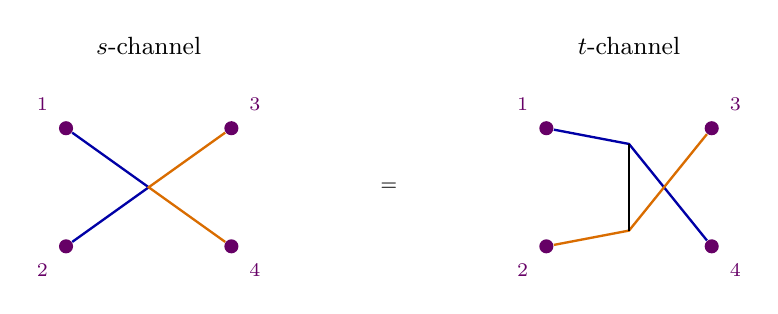
\begin{tikzpicture}[x=1cm,y=1cm,every node/.style={font=\scriptsize}]
    \tikzset{
      insertion/.style={circle,fill=violet!80!black,inner sep=1.8pt},
      line/.style={line width=0.85pt},
      arrow/.style={-{Latex[length=2mm]},line width=0.8pt}
    }
    \begin{scope}
      \node[font=\small] at (0,1.8) {\(s\)-channel};
      \node[insertion] (a) at (-1.05,0.75) {};
      \node[insertion] (b) at (-1.05,-0.75) {};
      \node[insertion] (c) at (1.05,0.75) {};
      \node[insertion] (d) at (1.05,-0.75) {};
      \draw[line,blue!65!black] (a)--(0,0)--(b);
      \draw[line,orange!85!black] (c)--(0,0)--(d);
      \node[violet!80!black] at (-1.35,1.05) {\(1\)};
      \node[violet!80!black] at (-1.35,-1.05) {\(2\)};
      \node[violet!80!black] at (1.35,1.05) {\(3\)};
      \node[violet!80!black] at (1.35,-1.05) {\(4\)};
    \end{scope}

    \node at (3.05,0) {\(=\)};

    \begin{scope}[shift={(6.10,0)}]
      \node[font=\small] at (0,1.8) {\(t\)-channel};
      \node[insertion] (a) at (-1.05,0.75) {};
      \node[insertion] (b) at (-1.05,-0.75) {};
      \node[insertion] (c) at (1.05,0.75) {};
      \node[insertion] (d) at (1.05,-0.75) {};
      \draw[line,blue!65!black] (a)--(0,0.55)--(d);
      \draw[line,orange!85!black] (b)--(0,-0.55)--(c);
      \draw[line] (0,0.55)--(0,-0.55);
      \node[violet!80!black] at (-1.35,1.05) {\(1\)};
      \node[violet!80!black] at (-1.35,-1.05) {\(2\)};
      \node[violet!80!black] at (1.35,1.05) {\(3\)};
      \node[violet!80!black] at (1.35,-1.05) {\(4\)};
    \end{scope}
  \end{tikzpicture}
  }
  \caption{Crossing symmetry states that different OPE decompositions of the
  same four-point function agree.}
  \label{fig:crossing-channels}
\end{figure}

\section{Linear Functionals}

Define the crossing vector
\[
  H_{\Delta,\ell}(u,v)
  =
  v^{\Delta_\phi}G_{\Delta,\ell}(u,v)
  -
  u^{\Delta_\phi}G_{\Delta,\ell}(v,u),
\]
and
\[
  H_{\mathbf 1}(u,v)=v^{\Delta_\phi}-u^{\Delta_\phi}.
\]
The crossing equation is
\begin{equation}
  H_{\mathbf 1}
  +
  \sum_{\mathcal O\ne\mathbf 1}
  \lambda_{\phi\phi\mathcal O}^2 H_{\Delta,\ell}=0.
  \label{eq:crossing-vector-form}
\end{equation}
A linear functional \(\alpha\) acting on functions of \(z,\bar z\) can rule
out a proposed spectrum if
\[
  \alpha(H_{\mathbf 1})<0,
  \qquad
  \alpha(H_{\Delta,\ell})\ge0
\]
for every nonidentity operator allowed by the proposal.  Applying \(\alpha\)
to \eqref{eq:crossing-vector-form} gives a contradiction because the OPE
coefficients are nonnegative.

This is the conceptual core of the numerical conformal bootstrap.  A finite
calculation chooses a finite-dimensional space of derivatives at the
crossing-symmetric point and searches for such a functional.  When the
functional is found with controlled numerical precision, the corresponding
spectral assumption is excluded.

The same method bounds OPE coefficients.  If the goal is to bound the
coefficient of a particular primary \((\Delta_\ast,\ell_\ast)\), one imposes
\[
  \alpha(H_{\Delta_\ast,\ell_\ast})=1,
  \qquad
  \alpha(H_{\Delta,\ell})\ge0
\]
on the remaining allowed operators.  Then
\[
  \lambda_{\phi\phi\mathcal O_\ast}^2
  \le
  -\alpha(H_{\mathbf1})
\]
after minimizing the right side over admissible functionals.  For
\(\mathcal O_\ast=T_{\mu\nu}\), this gives a lower bound on \(C_T\), since
the Ward identity fixes \(\lambda_{\phi\phi T}^2\) in terms of
\(\Delta_\phi^2/C_T\).
